\documentclass[color=usenames,dvipsnames]{beamer}\usepackage[]{graphicx}\usepackage[]{color}
% maxwidth is the original width if it is less than linewidth
% otherwise use linewidth (to make sure the graphics do not exceed the margin)
\makeatletter
\def\maxwidth{ %
  \ifdim\Gin@nat@width>\linewidth
    \linewidth
  \else
    \Gin@nat@width
  \fi
}
\makeatother

\definecolor{fgcolor}{rgb}{0.345, 0.345, 0.345}
\makeatletter
\@ifundefined{AddToHook}{}{\AddToHook{package/xcolor/after}{\definecolor{fgcolor}{rgb}{0.345, 0.345, 0.345}}}
\makeatother
\newcommand{\hlnum}[1]{\textcolor[rgb]{0.686,0.059,0.569}{#1}}%
\newcommand{\hlstr}[1]{\textcolor[rgb]{0.192,0.494,0.8}{#1}}%
\newcommand{\hlcom}[1]{\textcolor[rgb]{0.678,0.584,0.686}{\textit{#1}}}%
\newcommand{\hlopt}[1]{\textcolor[rgb]{0,0,0}{#1}}%
\newcommand{\hlstd}[1]{\textcolor[rgb]{0.345,0.345,0.345}{#1}}%
\newcommand{\hlkwa}[1]{\textcolor[rgb]{0.161,0.373,0.58}{\textbf{#1}}}%
\newcommand{\hlkwb}[1]{\textcolor[rgb]{0.69,0.353,0.396}{#1}}%
\newcommand{\hlkwc}[1]{\textcolor[rgb]{0.333,0.667,0.333}{#1}}%
\newcommand{\hlkwd}[1]{\textcolor[rgb]{0.737,0.353,0.396}{\textbf{#1}}}%
\let\hlipl\hlkwb

\usepackage{framed}
\makeatletter
\newenvironment{kframe}{%
 \def\at@end@of@kframe{}%
 \ifinner\ifhmode%
  \def\at@end@of@kframe{\end{minipage}}%
  \begin{minipage}{\columnwidth}%
 \fi\fi%
 \def\FrameCommand##1{\hskip\@totalleftmargin \hskip-\fboxsep
 \colorbox{shadecolor}{##1}\hskip-\fboxsep
     % There is no \\@totalrightmargin, so:
     \hskip-\linewidth \hskip-\@totalleftmargin \hskip\columnwidth}%
 \MakeFramed {\advance\hsize-\width
   \@totalleftmargin\z@ \linewidth\hsize
   \@setminipage}}%
 {\par\unskip\endMakeFramed%
 \at@end@of@kframe}
\makeatother

\definecolor{shadecolor}{rgb}{.97, .97, .97}
\definecolor{messagecolor}{rgb}{0, 0, 0}
\definecolor{warningcolor}{rgb}{1, 0, 1}
\definecolor{errorcolor}{rgb}{1, 0, 0}
\makeatletter
\@ifundefined{AddToHook}{}{\AddToHook{package/xcolor/after}{
\definecolor{shadecolor}{rgb}{.97, .97, .97}
\definecolor{messagecolor}{rgb}{0, 0, 0}
\definecolor{warningcolor}{rgb}{1, 0, 1}
\definecolor{errorcolor}{rgb}{1, 0, 0}
}}
\makeatother
\newenvironment{knitrout}{}{} % an empty environment to be redefined in TeX

\usepackage{alltt}
%\documentclass[color=usenames,dvipsnames,handout]{beamer}

%%\usepackage[roman]{../pres1}
\usepackage[sans]{../pres1}
\usepackage{graphicx}
\usepackage{bm}




\IfFileExists{upquote.sty}{\usepackage{upquote}}{}
\begin{document}


\begin{frame}[plain,fragile]
  \centering
    \huge
    The BIDE model \\
%    \large
%    January 14, 2019 \\
    \vfill

\begin{columns}
  \column{\dimexpr\paperwidth-10pt}
  \centering
  \includegraphics[width=0.75\textwidth]{figure/bide0-1} \\
\end{columns}
\end{frame}



\section{Definitions}


\begin{frame}
  \frametitle{Today's topics}
  \LARGE
  \only<1>{\tableofcontents}%[hideallsubsections]}
\end{frame}


\begin{frame}
  \frametitle{Definitions}
  {\bf Population dynamics \\}
    The study of spatial and temporal variation in population size and structure
  \pause
  \vfill
  {\bf Population \\}
    Individuals of the same species occuring in the same geographic region
  \pause
  \vfill
  {\bf Population size and structure \\}
    {\color{Red}
      \it Size:} Abundance \\
    {\color{Red}
      \it Structure:} Distribution of individuals among age groups, sexes,
    habitat patches, etc\dots
\end{frame}



\section{Modeling 101}





\begin{frame}
  \frametitle{Models and science}
  \large
  A model is an abstraction of reality that describes the relationship between two or more variables. \par
  \pause
  \vfill
%  \Large
  {%\bf
    Models help us\dots}
  \begin{itemize}[<+->]
    \item Describe complex natural systems in a manageable way
    \item Formalize and evaluate hypotheses
%    \item Evaluate hypotheses while accounting for uncertainty
    \item Predict future outcomes
    \item \dots all while accounting for uncertainty
  \end{itemize}
\end{frame}




\begin{frame}
  \frametitle{Models and science}
  \large
  {\it But don't models require assumptions?}
  \pause
  \vfill
  Yes. We have to simplify, so we have to make assumptions.
  \pause
  \vfill
  We do this all the time, for example when deciding how long it will take you to get to class. 
  \pause
  \vfill
  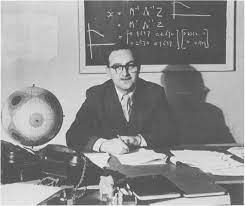
\includegraphics[width=0.3\textwidth]{figs/box}
  ``All models are wrong, but some are useful.'' G.E.P. Box (1987)
\end{frame}




\begin{frame}
  \frametitle{Model validation}
  \large
  {%\bf
    Putting the model to the test}
  \begin{itemize}[<+->]
    \item How well does it predict?
    \item Will your results hold up in court?
    \item Can your results be replicated/reproduced?
  \end{itemize}
\end{frame}


%\section{Modeling 101}




\begin{frame}
  \frametitle{Types of models}
  \Large
  \begin{itemize}
    \item {\color<2>{Red} Conceptual}
    \item Physical
    \item Graphical
%    \item {\color<2>[rgb]{0,0,1} Mathematical}
    \item {\color<2>{Red} Mathematical}
    \item {\color<2>{Red} Statistical}
  \end{itemize}
\end{frame}





\section{BIDE}


\begin{frame}
  \frametitle{The BIDE model}
  \huge
  \[
  N_{t+1} = N_t + B_t + I_t - D_t - E_t
  \]
  \large
  \vfill
%  \centering where \flushleft \par
  \centering \rule{4cm}{1pt} \flushleft \par
  \vfill
  \Large
  $N_t$: population size (state variable) at time $t$ \\
  $B_t$: births \\
  $I_t$: immigrants \\
  $D_t$: deaths \\
  $E_t$: emigrants
  \note{Ask students to write a factor that could influence each parameter}
  \note{Classify each variable: attributes of the animal, other biotic
    factors e.g. competitors/prey, attributes of the habitat, and population}
\end{frame}


\begin{frame}
  \frametitle{The BIDE model}
  \huge
  \[
  N_{t+1} = N_t + B_t + I_t - D_t - E_t
  \]
  \large
  \vfill
  {%\bf
    As written, this model implies the following:}
  \begin{itemize}%[<+->]
    \item<1-> $B$, $I$, $D$, and $E$ are not rates, they
      are the number of events at time $t$.
    \item The model is {\bf deterministic}, not {\bf stochastic}
    \item Time is discrete, not continuous
  \end{itemize}
%  \vspace{0.5cm}
  \pause
  \vfill
  % \bf
  In reality, things are more complicated, and interest lies in
  understanding the factors influencing each process.\par
  \pause
  \vfill
  % {\bf Group exercise:} Break into teams of 4-5 and create list of factors influenceing B, I, D, and E. 
  \note{Spend the rest of lecture doing a group exercise to create
    list of factors influencing each process?}
\end{frame}


\begin{frame}
  \frametitle{The BIDE model}
  \begin{columns}
    \column{\dimexpr\paperwidth-10pt}
    \centering
    \includegraphics[width=0.75\textwidth]{figure/bide0-1} \\
  \end{columns}
\end{frame}


\section{Assignment}


\begin{frame}
  \frametitle{Assignment}
  \large
%  \bf
  Read the first 3 pages of Chapter 3 in Conroy and Carroll \\
  \vfill
  Expect a quiz next time we meet
\end{frame}







\end{document}
